% Content for the test report for LSP-00-20

\subsection{Portal Aspect tests}

This test case exercises the LSP via the Portal Aspect only,
though it depends on the API Aspect for its operation.

It verifies the ability to perform a variety of display and exploratory data analysis
operations in the Portal Aspect UI.
Data for the test are taken from the Object-like AllWISE (coadded) Source Catalog.

\subsubsection{Step 1}

The tests were performed primarily from an Apple MacBook Pro laptop computer running OS X 10.12.6,
connected to the Internet using a wired connection to the IPAC institutional network.
The Portal was accessed using the Google Chrome browser, version 66.0.3359.139.

\subsubsection{Step 2}

A connection was established to the PDAC network environment using the NCSA VPN at \texttt{vpn.ncsa.illinois.edu}.

\subsubsection{Step 3}

\textbf{Step 3a:} The Portal was accessed at:

\begin{center}
\texttt{https://lsst-sui-proxy01.ncsa.illinois.edu/suit/}
\end{center}

\textbf{Step 3b:} The test case instructs that a cone search returning at least 10,000 records be performed.
In practice there are two problems with this:

\begin{enumerate}
\item{The Portal interface limits cone searches to the rather tiny radius of 100 arcseconds,
which in the AllWISE dataset cannot come close to yielding that many records.}
\item{The Portal limits scatterplots to a maximum of 5,000 points before falling back to representing the data as a 2D histogram or ``heat map''.}
\end{enumerate}

Neither of these limits is functionally essential.
The Portal and the underlying DAX and Qserv interfaces can handle much larger search areas while preserving good performance.
The polygon search interface exposed by the Portal can be used to query much larger areas while still yielding latencies compatible with interactive work, as noted in LSP-00-15 above,
so there is no reason to limit the cone search so dramatically.
For example, an XXX sq. deg. polygon search in the Object-like AllWISE Source Catalog executes in YYY seconds, and the resulting ZZZ row result table can be browsed and analyzed interactively with good performance.

The limit on the scatterplot density is also overly conservative, though not by as large a factor.
The current \verb|Plotly| implementation begins to slow down significantly when more than 20,000 points are displayed.
The scatterplot limit has recently been raised in IRSA production, and there is no reason not to do this in LSST.

In addition, as described in the Summary section above, an alternate \verb|Plotly| implementation, based on WebGL, is available which should scale to much larger plots.

Nevertheless, given the limits observed, the test case actually executed was modified as follows to permit all the remaining steps in the test case to function without further restrictions:

\begin{itemize}
\item{a polygon search was used in place of a cone search, in order to permit searching a larger area; and}
\item{the number of rows returned was adjusted to keep it below 5,000.}
\end{itemize}

The resulting query, used as the input to the remaining steps in this section,
was to select the polygonal region \{ (281.7, -2.4), (281.7, -2.8), (281.3, -2.8), (281.3, -2.4) \} from the AllWISE Source Catalog,
an area of approximately 0.16 square degrees.
This search yielded 3,479 objects.
The search was restricted via GUI to a subset of the available columns.

\begin{figure}
  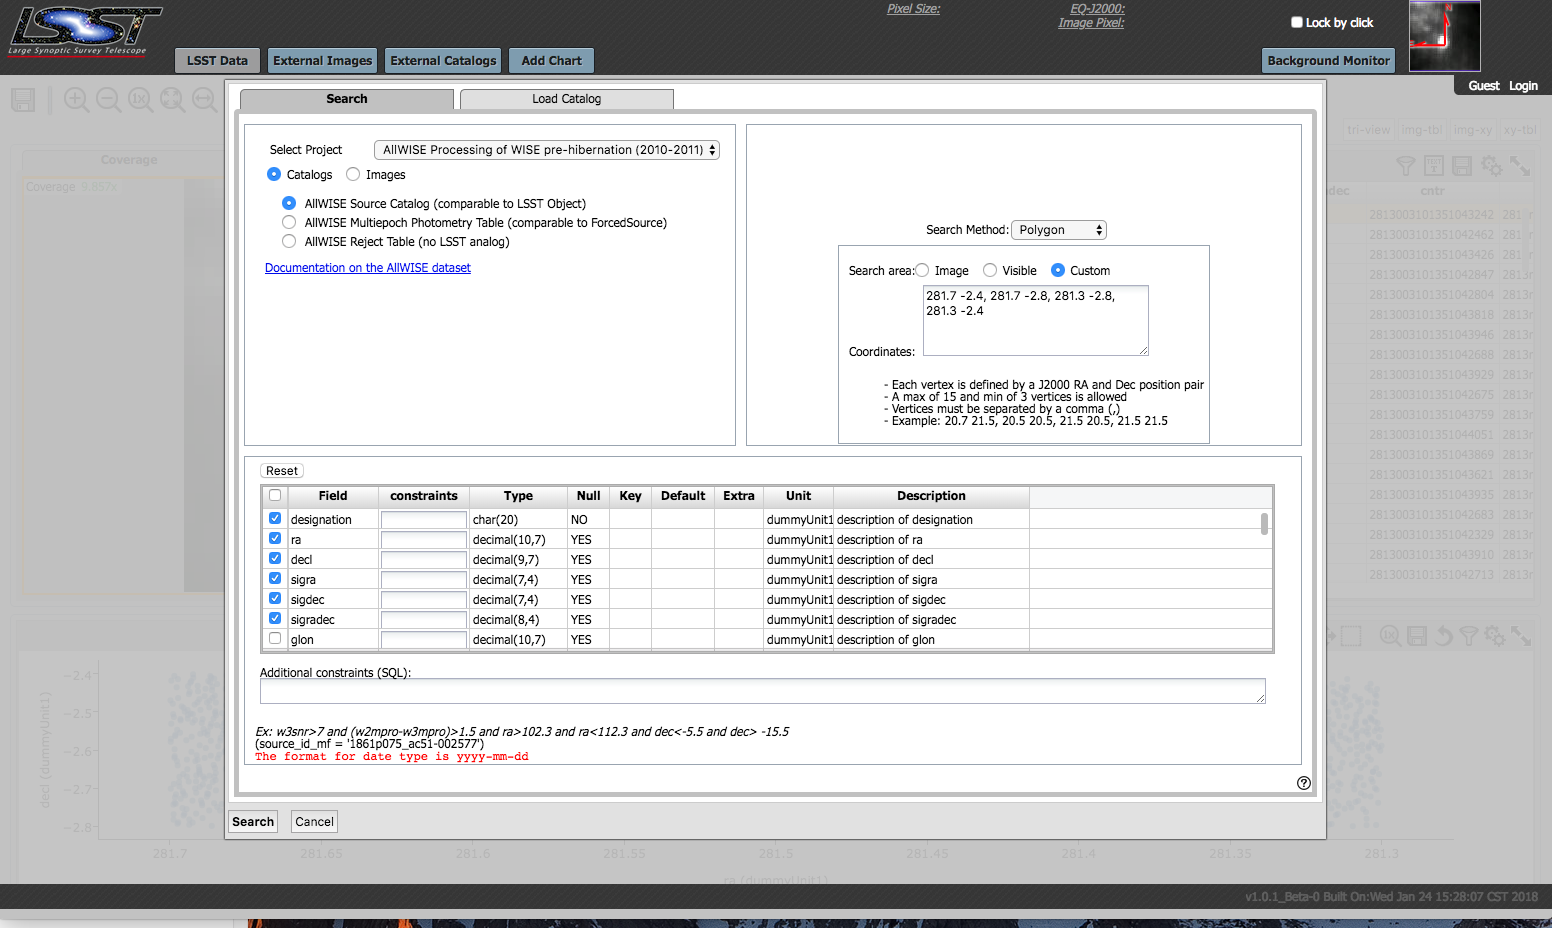
\includegraphics[width=\linewidth]{lsp-00-20/step3Search_a.png}
  \caption{Query screen for the Object-like AllWISE Source Catalog}
  \label{fig:lsp-00-20-search}
\end{figure}

\begin{figure}
  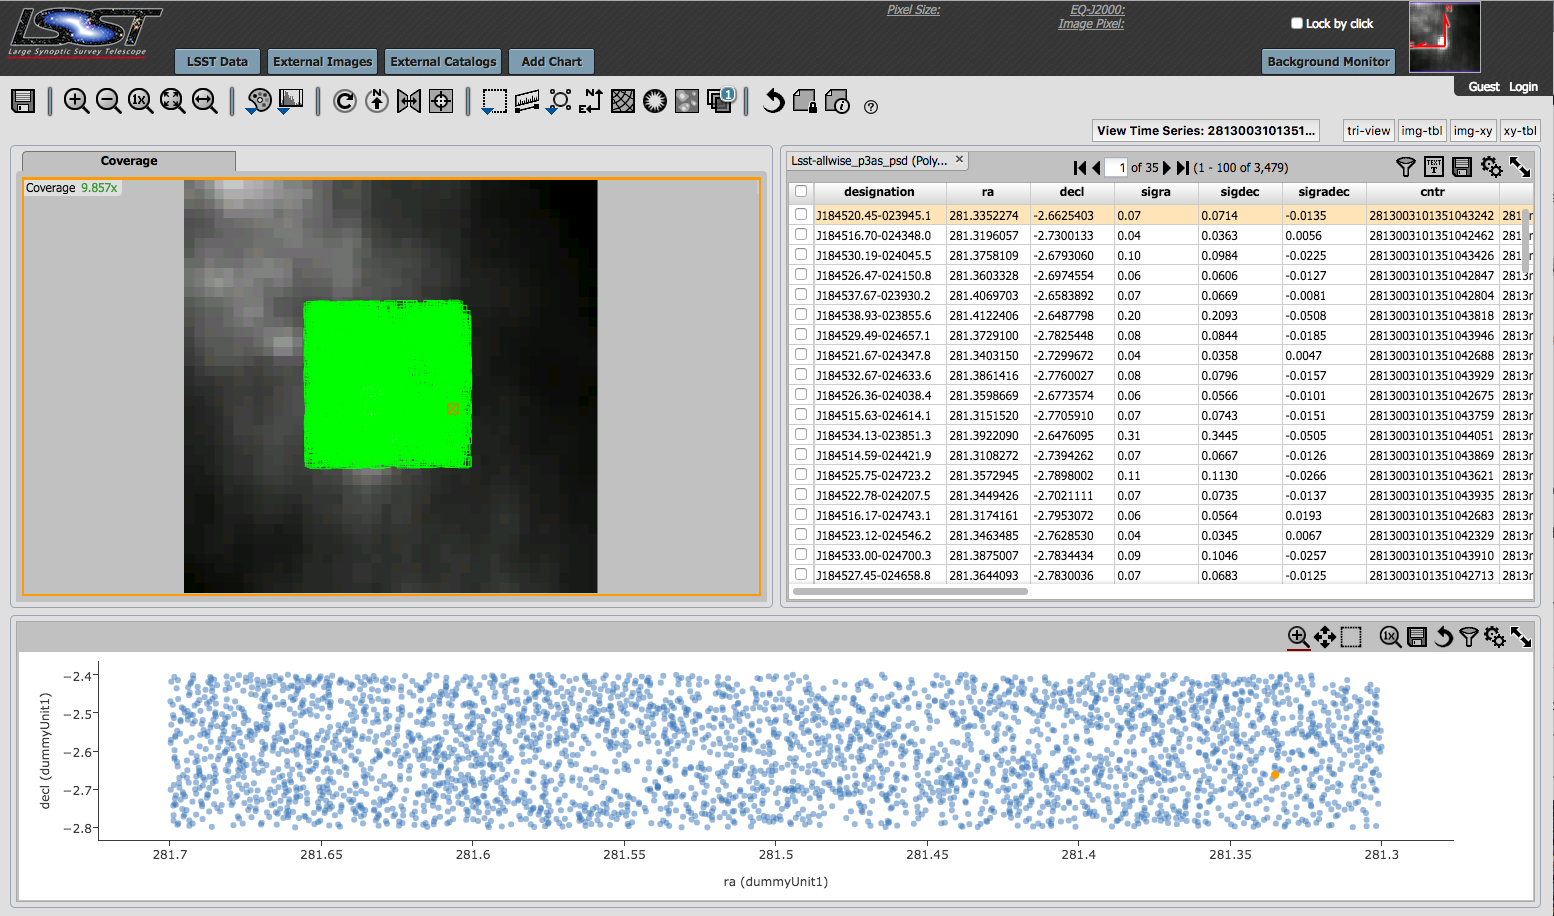
\includegraphics[width=\linewidth]{lsp-00-20/step3Result_a.png}
  \caption{Result screen for the Object-like search near M81}
  \label{fig:lsp-00-20-result-table}
\end{figure}

\textbf{Step 3c:} The table-download feature of the UI was used to produce the file preserved as \verb|DMTR-52/lsp-00-20/step3-c.tbl|.
No choice of file types was offered.
The format is IPAC Table, with 17 rows of metadata and the expected 3,479 rows of data.

The table was confirmed by inspection of the first and last three rows in the GUI to be in the same basic order as displayed in the GUI.

The table was verified programmatically to contain \verb|ra| and \verb|decl| values well-distributed right up to the specified limits of the query,
with the extrema being \{281.3000661, 281.6998140\} and \{-2.7998067, -2.4000119\},
respectively.
No attempt was made to determine whether this was consistent with expected spherical-geometry deviations from the region boundaries,
given the small size of the region.

\textbf{Step 3d:} The UI was used to sort the table based on the numeric column \verb|ra|,
and the result was visually inspected to be sorted as requested.
Both sort directions were tested in the UI.
The table, sorted in ascending \verb|ra| order, was downloaded as \verb|DMTR-52/lsp-00-20/step3-d.tbl|.

The UI was then used to sort the table based on the string column \verb|description|,
with the table downloaded in ascending-\verb|description| order as \verb|DMTR-52/lsp-00-20/step3-d2.tbl|.

\textbf{Step 3e:} The sort order for the numeric \verb|ra| column was confirmed by testing with the POSIX \texttt{sort -gs} utility on MacOS 10.11.6.
The \verb|-s| (``stable'') option was required because of the presence of rows in which the \verb|ra| values were identical to the 10 significant digits provided.

The sort order for the string column \verb|description| was similarly verified with POSIX \verb|sort| applied to the downloaded file.

It was noted that the downloaded table files contain an additional column \verb|ROW_IDX| which contains a sequential index of the rows resulting from the initial query.
These are preserved across sorting and filtering.

\textbf{Step 3f:} The UI was used to perform an interactive filtering operation on the resulting table,
applying the filter \verb|sigdec| $> 0.4$.
The distribution of this variable is shown below; the filter selected only 28 of the 3,479 rows.

\begin{figure}
  \centering
  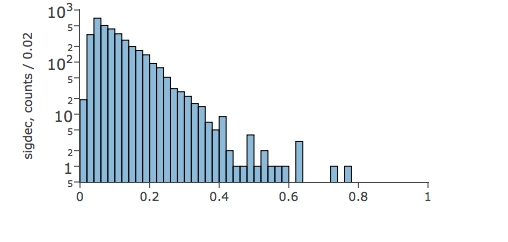
\includegraphics[width=4in]{lsp-00-20/step3-f-sigdec-hist.png}
  \caption{Histogram of \texttt{sigdec} before Step 3f filter}
  \label{fig:lsp-00-20-sigdec-hist}
\end{figure}

Visual inspection confirmed that the remaining rows all satisfied the filter.
The filtered result was downloaded as \verb|DMTR-52/lsp-00-20/step3-f.tbl|,
and was confirmed to contain only the displayed rows.
The POSIX \verb|awk| utility was used to apply the same selection independently to the original download from Step 3c,
and verify that the same rows were selected as by the filter in the UI.

\begin{figure}
  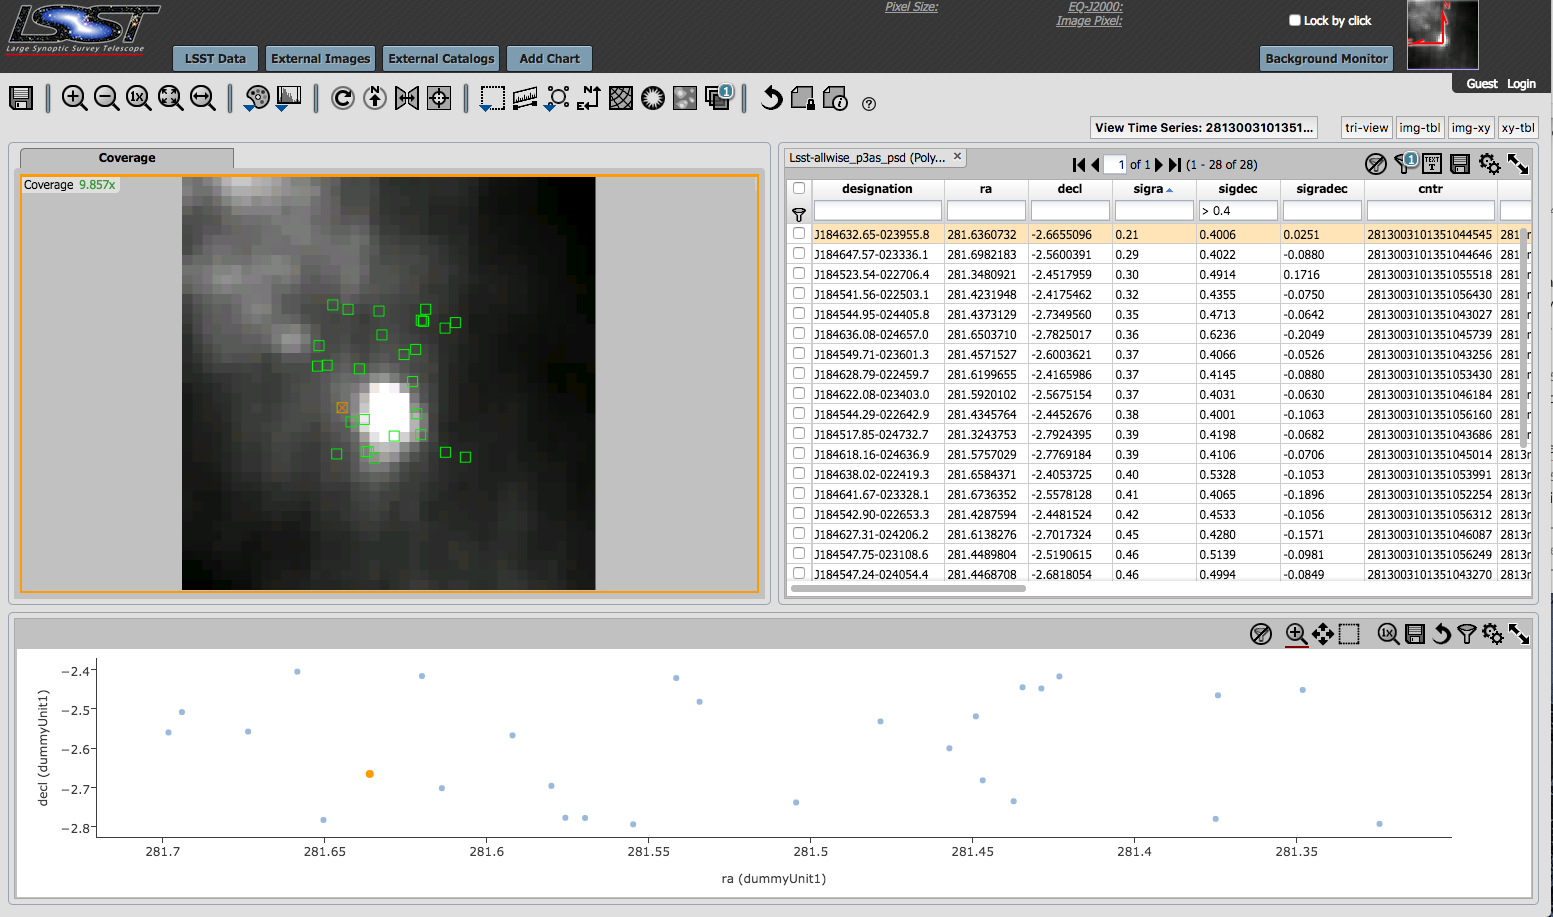
\includegraphics[width=\linewidth]{lsp-00-20/step3-f.png}
  \caption{UI following application of filter on \texttt{sigdec}}
  \label{fig:lsp-00-20-sigdec-filter}
\end{figure}

\textbf{Step 3g:} Four rows were manually selected using the UI checkboxes,
and then the table was filtered on these selections.
The resulting four-row table was downloaded and visually confirmed to contain the same rows as displayed in the UI.

\textbf{Step 3h:} The UI was used to create a 1D histogram of \verb|sigdec|, as displayed above in Figure~\ref{fig:lsp-00-20-sigdec-hist}.
Hovering over selected bins, and noting the bin count reported, \verb|awk| was used on the table from Step 3c above to verify the count.
The limited number of significant figures reported for \verb|sigdec| facilitated verifying that the bin definitions are inclusive on the low side and exclusive on the high side, as is conventional.

\begin{figure}
  \centering
  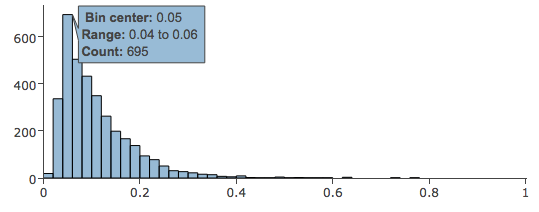
\includegraphics[width=4in]{lsp-00-20/step3-h-hover.png}
  \caption{Histogram of \texttt{sigdec}, showing hover text for a bin}
  \label{fig:lsp-00-20-sigdec-hist-hover}
\end{figure}

\textbf{Step 3i:} The UI was used to create a 2D histogram or ``heat map'' of \verb|sigra| and \verb|sigdec|.
The spot checks in the test specification were performed to validate that outlying points in the distribution were displayed where expected.
However, the combination of the hover text information displayed and the limited ability to control the bin boundaries meant that it was difficult to perform a quantitative verification of the binning itself.
As noted in the summary above, while adequate to pass this early test, improvements are needed in order to support serious quantitative usage of this feature.

\begin{figure}
  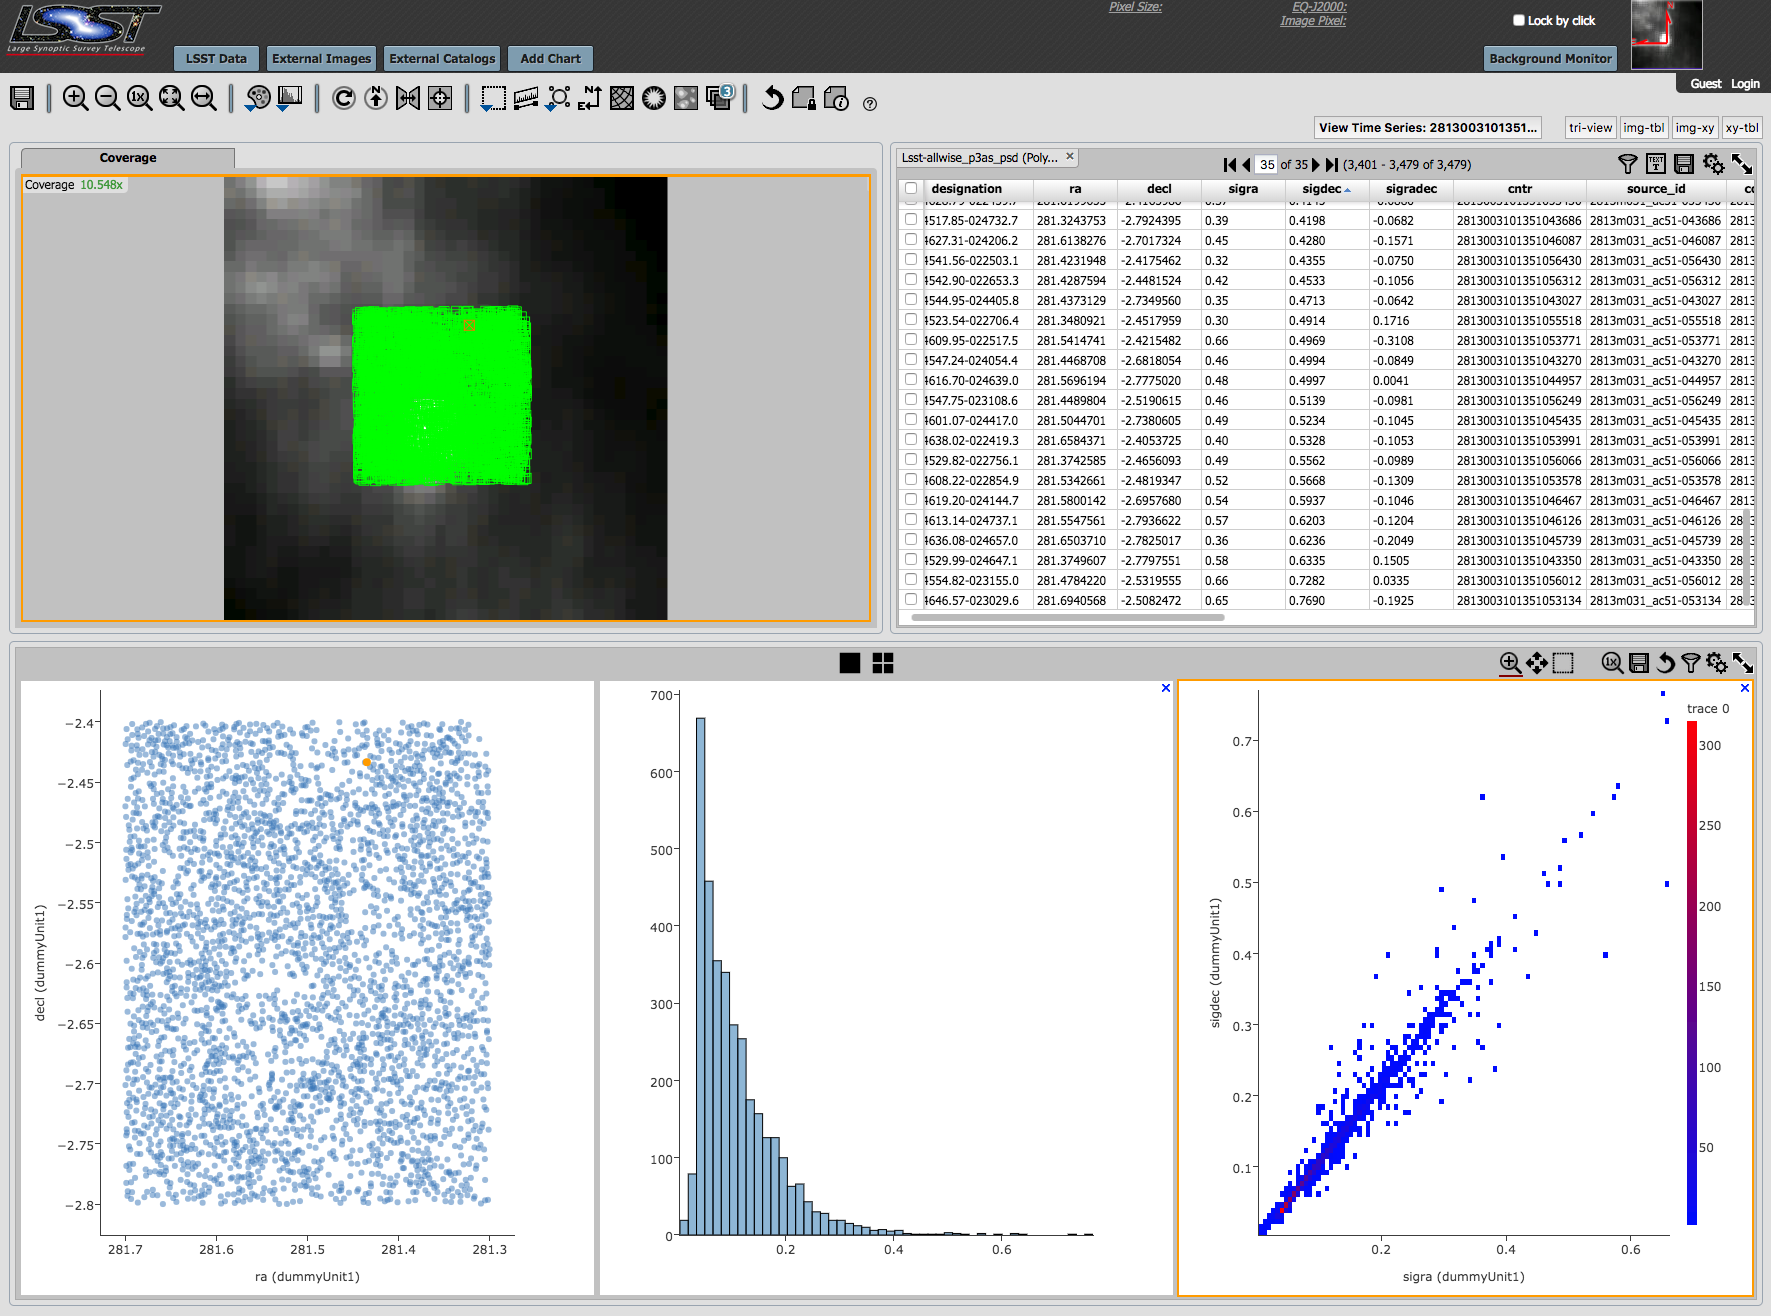
\includegraphics[width=\linewidth]{lsp-00-20/step3-i.png}
  \caption{UI showing 1D and 2D histograms.}
  \label{fig:lsp-00-20-2Dhist}
\end{figure}

\textbf{Step 3j:} The UI was used to draw a rectangular selection on a scatterplot of \verb|ra| versus \verb|dec|,
with the approximate limits, judged from the UI, of \{~\{281.465, 281.58\}, \{-2.665, -2.595\}~\}.
The UI did not provide the expected means of reading off the exact boundaries once the region had been established.

\begin{figure}
  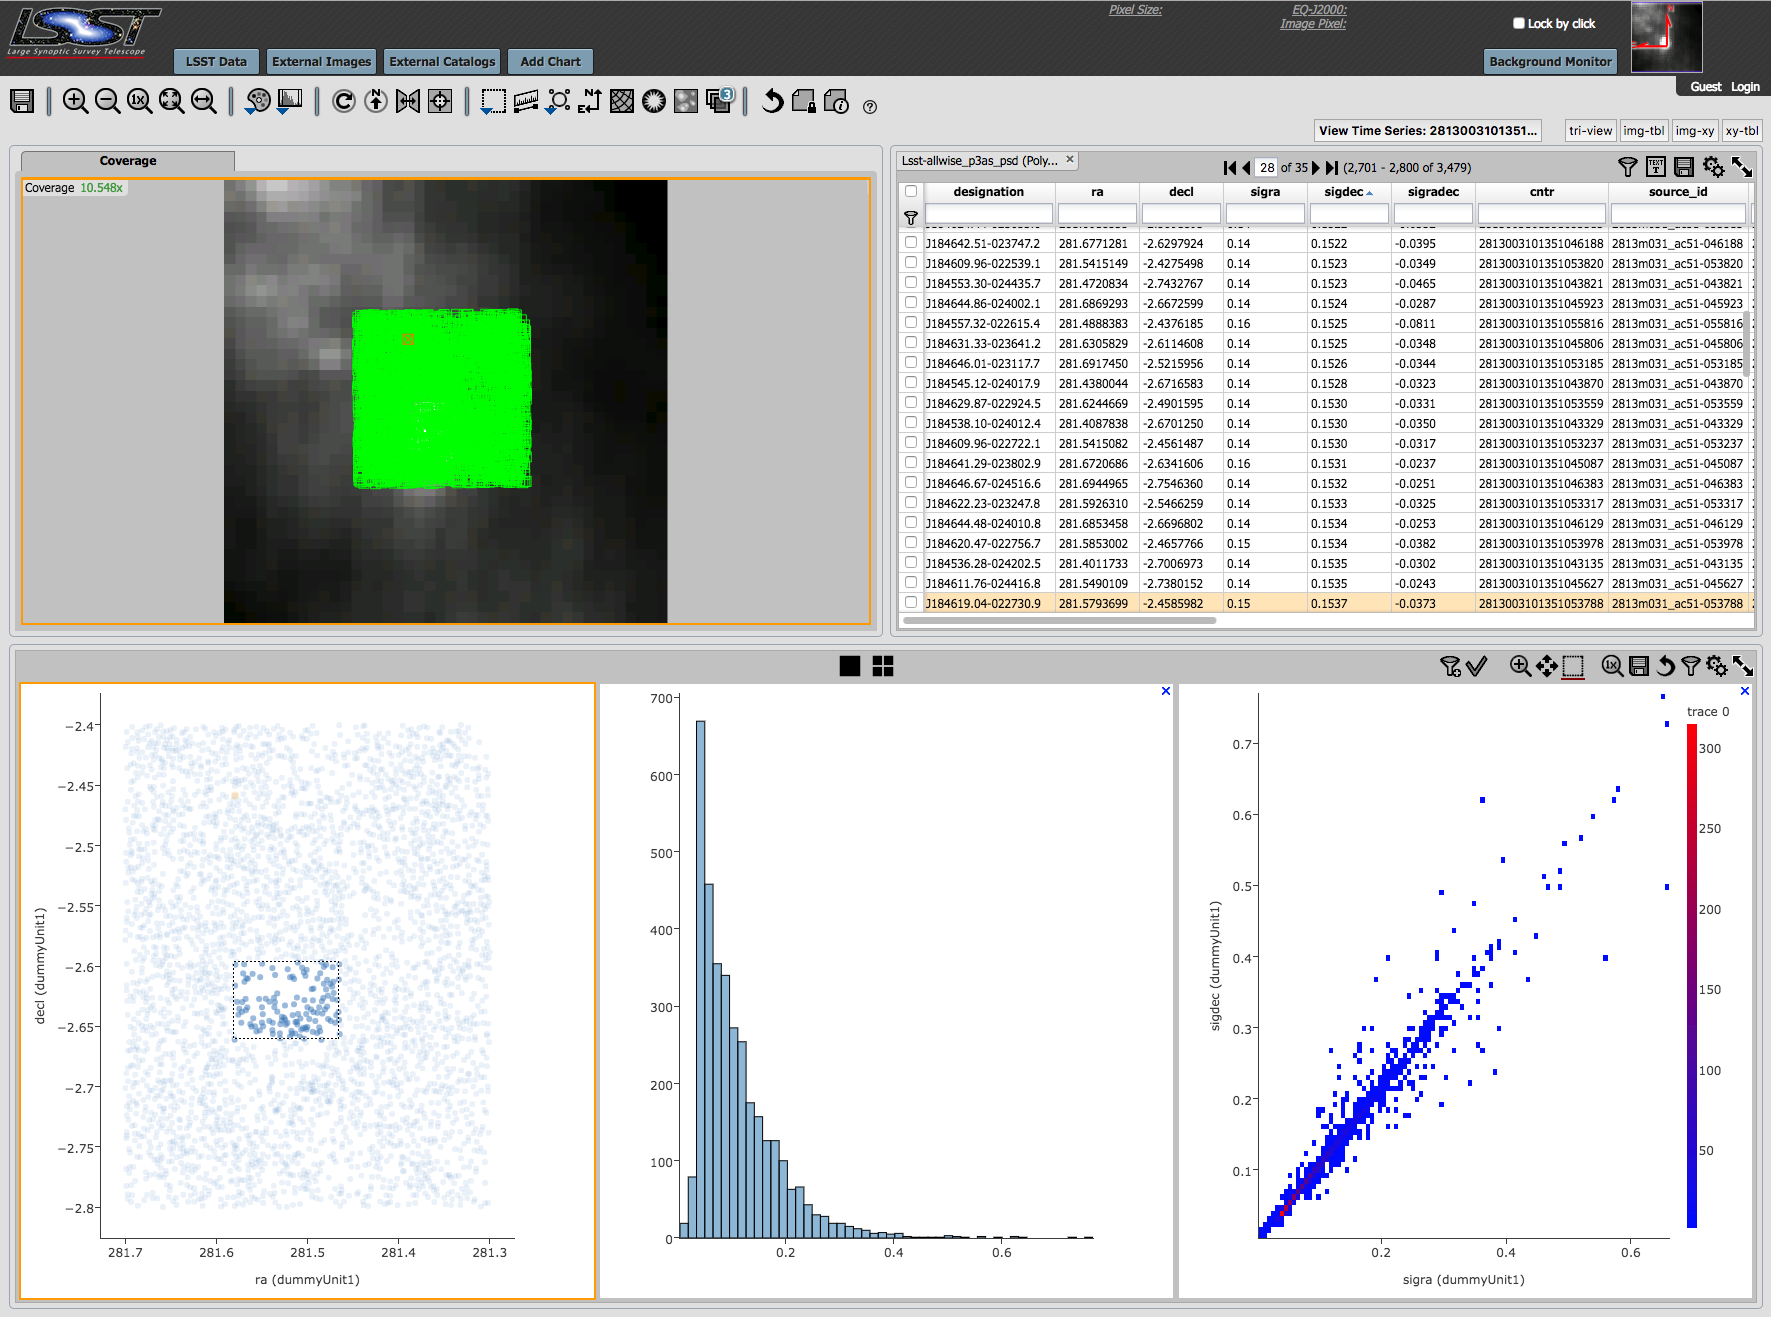
\includegraphics[width=\linewidth]{lsp-00-20/step3-j.png}
  \caption{Step 3j selection region being drawn.}
  \label{fig:lsp-00-20-rect-selecting}
\end{figure}

\begin{figure}
  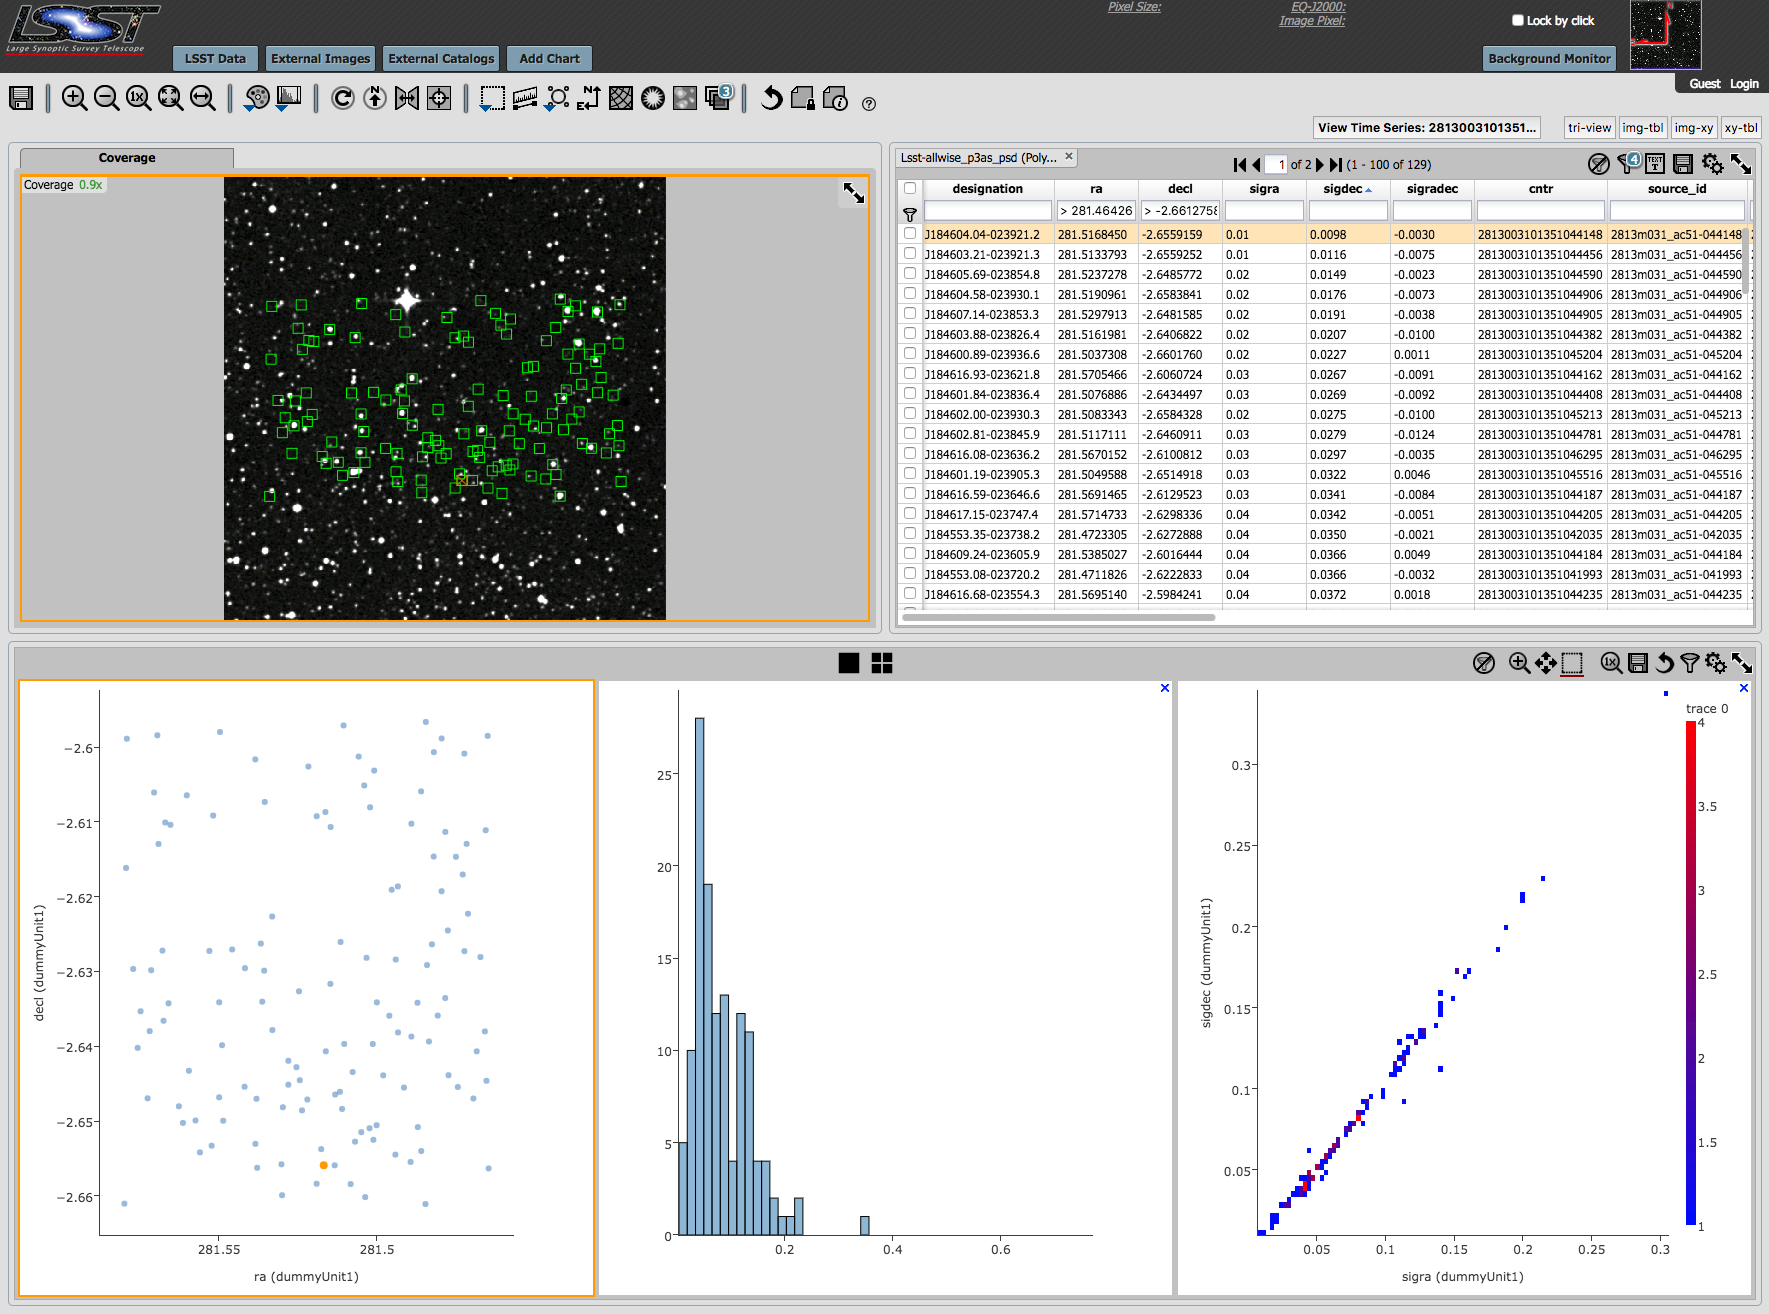
\includegraphics[width=\linewidth]{lsp-00-20/step3-j2.png}
  \caption{Display following application of Step3j 2D selection.}
  \label{fig:lsp-00-20-rect-selected}
\end{figure}

The filtered result, containing 129 rows, was downloaded as \verb|DMTR-52/lsp-00-20/step3-j.tbl|.
POSIX utilities were used to determine the extrema of the values of \verb|ra| and \verb|dec| for the selected rows:
\{281.4646684, 281.5799433\} and \{-2.6611025, -2.5966385\}, respectively.
This appears consistent, within the ability to read off from the original selection, with the bounds chosen.
